\chapter{Integrazione fra Back-end e Front-end}
\label{cap:chapter7}

\section{Programma MapEnumerator}

Sebbene tutte le mappe fossero state caricate all'interno di GeoSever, mediante l'utilizzo del programma AutoLoader, non esisteva alcun meccanismo, fino ad oggi, che informasse il front-end su quali fossero le mappe disponibili e che sistema usare per reperirle. Infatti, il codice esistente realizzato lato front-end prevedeva che si fosse già a conoscenza del tipo di mappa desiderata, oltre a possedere una struttura in cui veniva specificata esattamente la mappa da reperire, non permettendo così di supportare l'aggiunta di nuove mappe. 
\\In questa ultima fase di sviluppo, quindi, l'obiettivo del tirocinante è stato quello sia di realizzare una figura, lato back-end, che potesse memorizzare e comunicare tutte le mappe consultabili, sia quello di implementare, lato front-end, un codice che potesse leggere il contenuto della lista e poi mostrare le mappe a schermo.
\\~\\
L'idea principale per risolvere questo problema è stata quella di realizzare, lato back-end, un programma in C\# che potesse memorizzare all'interno di un database tutte le mappe. È stato poi creato, utilizzando lo standard REST API, un nuovo endpoint in cui fornire la lista completa in formato JSON. Si è poi fornita la possibilità al client di poter interrogare selettivamente la Rest API, facendo uso dei query params, per ottenere informazioni più specifiche (per esempio, chiedere un numero finito di mappe disponibili, oppure l'elenco di mappe filtrato per un certa caratteristica). 
\\Oltre che a fornire l'elenco dei nomi delle mappe, è stato ritenuto adeguato offrire ulteriori informazioni ad esse relative, come il tipo di proiezione geospaziale o il protocollo da utilizzare, così che la mappa potesse essere mostrata correttamente. Infine, questo meccanismo avrebbe dovuto fornire un elenco di mappe non esclusive a un singolo server, come nel caso di GeoServer, ma anche di ulteriori server esterni, come ad esempio la mappa di default fornita da OpenStreetMap. 
\\Per quanto riguarda il front-end, invece, si è preferito realizzare una nuova pagina, in cui richiedere l'elenco delle mappe in formato JSON e successivamente, sfruttando le informazioni ricevute, renderle utilizzabili all'utente.   

\subsection{Struttura del Database}

Il lavoro è dunque iniziato implementando all'interno del back-end un codice che permettesse di memorizzare in maniera persistente la lista delle mappe. Per fare ciò, sono state utilizzate delle librerie apposite fornite direttamente da .NET, le quali hanno permesso di eseguire operazioni sul database, senza la necessità di dover scrivere manualmente query in linguaggio SQL. Facendo uso della classe \verb|ApplicationContex|, la quale estendeva le funzionalità fornite da \verb|DbContext|, è stato quindi possibile creare in automatico una nuova tabella all'interno del database. Quest'ultima è stata realizzata, seguendo la struttura definita in un'altra classe (nota con il nome di \verb|GeoMap|), nel seguente modo:
\begin{itemize}
    \item \verb|Id|: è stato utilizzato come chiave primaria della tabella e conteneva al suo interno tutti gli ID delle mappe. Questi ultimi erano stati generati come GUID anziché come numeri auto incrementati;
    \item \verb|Name|: conteneva i nomi delle mappe che poi il front-end avrebbe utilizzato all'interno dell'applicazione;
    \item \verb|Format|: questo campo serviva per fornire informazioni sul tipo di protocollo da utilizzare al fine di richiedere la mappa correttamente;
    \item \verb|Tags|: questo campo, definito come un array di stringhe, consentiva di dare delle descrizioni sul tipo di mappa memorizzata. Ciò era essenziale per raggruppare le mappe in diverse categorie (come ad esempio "Rischio Frane", "Rischio Alluvioni", ecc..);
    \item \verb|Data|: siccome le informazioni necessarie al front-end per recuperare le mappe dal server variavano a seconda del protocollo scelto e poiché tali informazioni non erano utili al back-end per eseguire eventuali operazioni, è stato deciso di inserire tutte queste informazioni all'interno di un unico campo. Ad esempio, mentre una mappa poteva avere uno stile SLD applicato, un'altra poteva non averne e di conseguenza, i parametri della richiesta da inviare al server di mappe dovevano essere diversi, in modo da richiedere la mappa con lo stile applicato.
    \\Questo campo è stato definito come un oggetto JSON, differente per ogni mappa, che conteneva al suo interno tutte le informazioni necessarie per il front-end al fine di richiedere correttamente quella mappa. Il campo Data di una mappa in formato WMTS era il seguente:
    \begin{lstlisting}[language=Java]{}
    {
       "capabilitiesUrl":"/example.com/?service=WMTS&request=GetCapabilities",
       "layer":"my_layer_name",
       "matrixSet":"EPSG:4326"
    }
    \end{lstlisting}
    \item \verb|CreatedAt|: utilizzato per tenere traccia della data e dell'ora in cui la mappa era stata inserita nel database;
    \item \verb|UpdatedAt|: veniva utilizzato per tenere traccia dell'ultima modifica effettuata sulla riga del database relativa alla mappa;
\end{itemize}

\subsection{Inserimento delle mappe nel Database}

Per aggiungere le mappe all'interno del database, è stato deciso di creare un nuovo comando all'interno del back-end, anch'esso eseguibile tramite CLI. Questo comando, chiamato \verb|'to-database'|, richiedeva come input per il suo funzionamento un file CSV, in modo analogo al comando realizzato per l'AutoLoader.
Questo comando leggeva, in maniera asincrona, tutte le righe all'interno del file e per ognuna di esse creava una nuova entry all'interno del database. Tuttavia, il file utilizzato dal comando \verb|'to-geoserver'| (per caricare gli elementi all'interno del GeoServer), non coincideva con quello utilizzato dal nuovo comando, in quanto era necessario che questo file avesse una struttura analoga a quella della tabella del database.
\\Per realizzare il comando  \verb|'to-database'|, si è fatto nuovamente uso della libreria CSVHelper, la quale ha permesso di far leggere a tale comando il contenuto del file CSV. Purtroppo, tale libreria non supportava nativamente la deserializzazione e la serializzazione del JSON, non riuscendo quindi a estrapolare il contenuto della colonna Data. Per risolvere questo problema, è stato sufficiente introdurre un nuovo tipo di dato riconosciuto dalla libreria CsvHelper. Il tirocinante ha quindi creato una nuova classe che implementava l'interfaccia  \verb|ITypeConverter|, la quale richiedeva a sua volta l'implementazione di due nuovi metodi, uno utilizzato per la serializzazione e uno per la deserializzazione.
\\Per sincronizzare il contenuto delle mappe sul database con quello di GeoServer, il tirocinante ha infine modificato il comando \verb|'to-geoserver'| di modo che, dopo aver inserito le mappe all'interno di GeoServer, avrebbe poi restituito in standard output un nuovo file CSV compatibile con il comando \verb|'to-database'|. Quindi, era possibile eseguire, in sequenza, il comando \verb|'to-geoserver'|, per caricare delle mappe all'interno di GeoServer, e successivamente eseguire \verb|'to-database'|, così da avere le stesse mappe anche sul database.

\subsection{Creazione del servizio Rest API}

Una volta caricate le mappe all'interno del database, è stato quindi necessario realizzare un meccanismo che consentisse di pubblicarle al front-end. Per fare ciò, si è esteso il codice della Rest API già presente all'interno del progetto, avvalendosi delle stesse librerie (fornite dal framework .NET) da loro utilizzate. Precisamente, è stata realizzata una nuova classe, nota con il nome di GeoMapDto (Data Transfer Object), che veniva utilizzata per esporre la struttura della classe GeoMap al front-end. In questo modo, era quindi possibile fornire al front-end solamente una parte delle proprietà della classe GeoMap, mascherando tutte quelle che risultavano superflue al front-end.
\\Successivamente, è stato poi aggiunto un codice che permettesse di eseguire il mapping tra le due classi, riuscendo quindi a convertire un oggetto della classe GeoMapDto a GeoMap, e viceversa: in questo modo era quindi possibile ricevere i dati dal front-end mediante GeoMapDto, convertirli in un oggetto GeoMap e successivamente effettuare eventuali operazioni sul database; la stessa operazione si poteva svolgere anche nella direzione opposta, in modo tale che il back-end potesse inviare dati al front-end. 
\\Infine è stato aggiunto, all'interno della classe che si occupava di gestire tutti gli endpoint della Rest API, un nuovo endpoint apposito per le mappe. Quest'ultimo permetteva di far eseguire al front-end due tipi di richieste, entrambe in GET: la prima, permetteva di recuperare la lista di tutte le mappe disponibili, restituendo tutte le informazioni presenti nelle entries del database; la seconda, invece, permetteva di ricevere informazioni di una singola mappa, a patto che venisse specificato il suo identificativo (GUID). 
La rest API così realizzata rispettava lo standard di OpenAPI 3 e  forniva la sua documentazione attraverso SwaggerUI.
\medskip
\\Per verificare il funzionamento della Rest API, il tirocinante, facendo uso del framework Vitest, ha infine creato una nuova batteria di test che si sarebbe occupata di analizzare ed eseguire tutte le possibili operazioni che un client avrebbe potuto richiede all'endpoint delle mappe. Questi ultimi venivano eseguiti in sequenza ed includevano dei controlli come la quantità di mappe disponibili, la presenza di mappe con tag specifici, il recupero di un numero specifico di mappe, etc...

\subsection{Integrazione front-end della Rest API}

Terminata la parte di scrittura di codice relativa al back-end, il lavoro è poi proseguito verso l'integrazione nel front-end della Rest API, appena sviluppata. Il tirocinante ha scelto di creare una nuova pagina web all'interno dell'applicazione, anziché modificare la pagina, fino ad ora utilizzata, così da preservare il lavoro precedentemente svolto e avere entrambe le implementazioni funzionanti.
\\Innanzitutto, è stato fatto in modo che il front-end riuscisse a contattare il servizio di Rest API per ottenere la lista di mappe. Piuttosto che scrivere manualmente un codice che si occupasse di inviare richieste HTTP asincrone e che estrapolasse il contenuto delle risposte dal back-end, si è optato per l'utilizzo di una libreria apposita. Questa libreria (OpenAPI Generator), analizzando la specifica OpenAPI fornita dalla REST API stessa, permetteva di generare automaticamente del codice TypeScript per contattare il back-end. Da ciò è stato quindi possibile creare un servizio Angular che, utilizzando il codice auto generato, fornisse una serie di metodi utili sia per ottenere l'elenco di tutte le mappe disponibili, sia per ottenere le informazioni su una singola mappa. Questa implementazione, per rappresentare in memoria gli oggetti della mappa (ottenuti come risposta a eventuali richieste), utilizzava una classe che era identica a quella del GeoMapDto (lato back-end).
\\Il lavoro è poi continuato utilizzando i metodi forniti dal servizio Angular, così da riuscire ad inviare richieste HTTP al back-end. L'immagine \ref{fig:restAPI} mostra il contenuto, in formato JSON, della risposta inviata dal servizio di Rest API per ottenere l'elenco delle mappe. 
\begin{figure}[htbp]
      \centering
      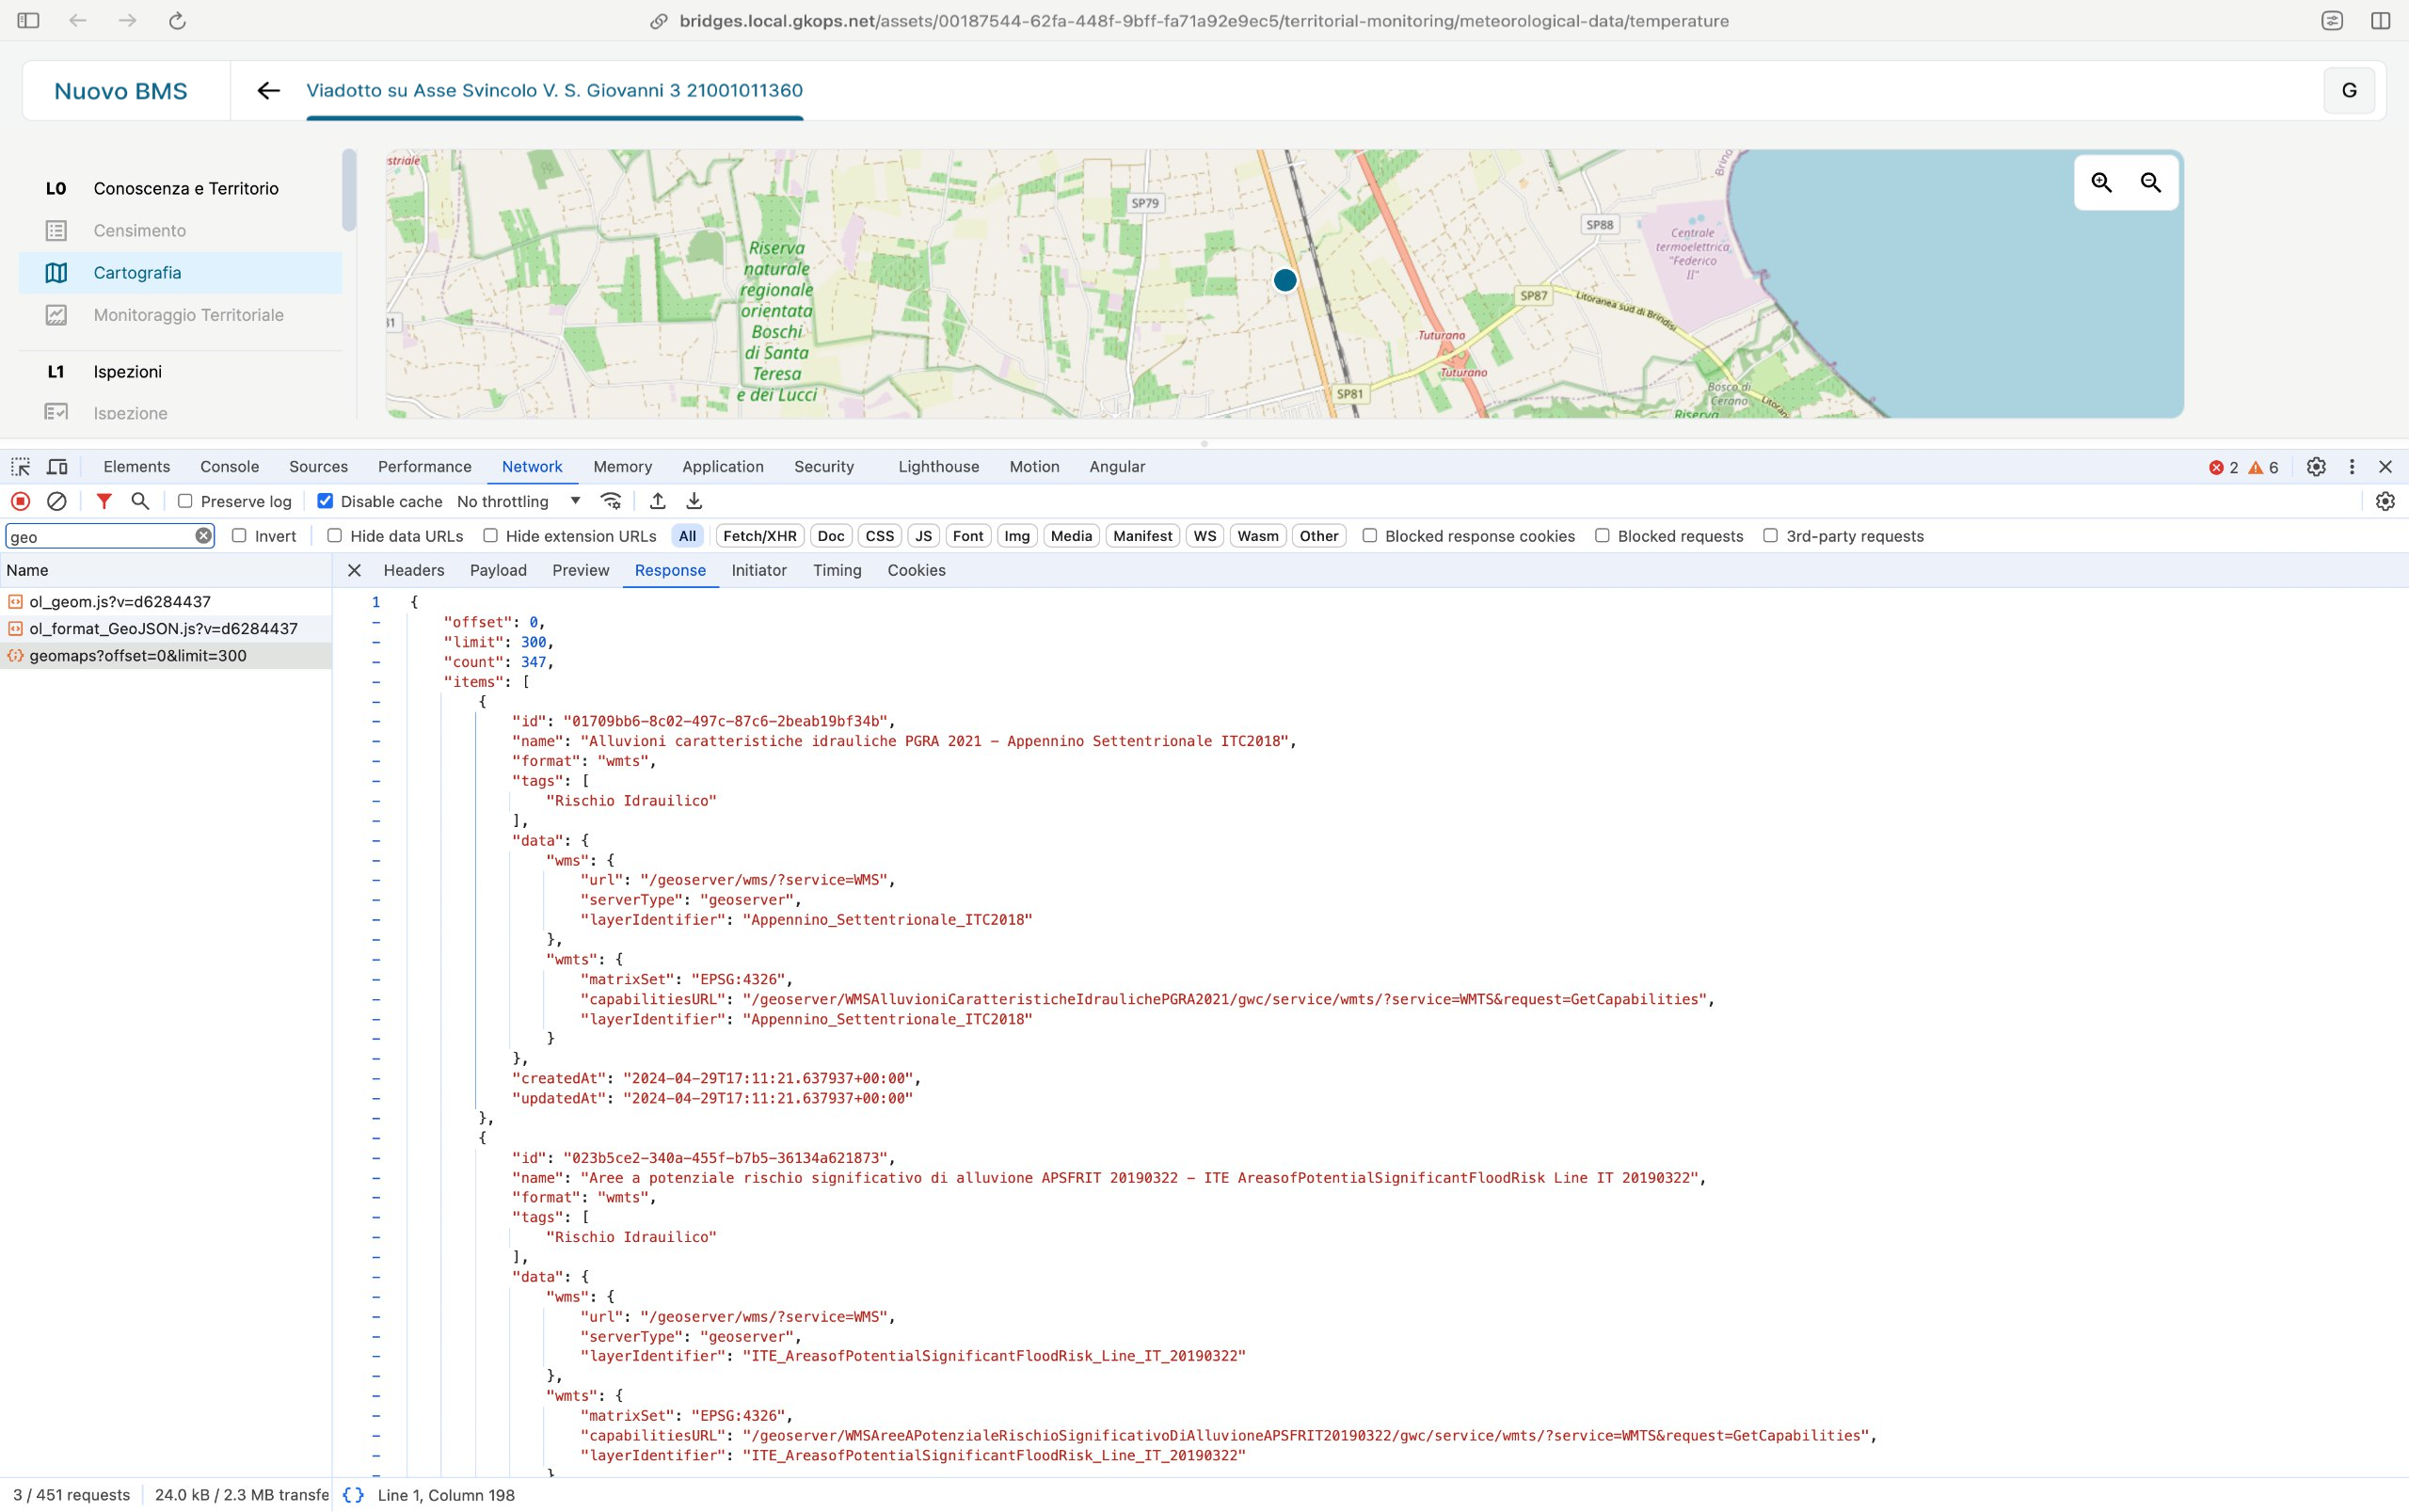
\includegraphics[width=1\textwidth]{Tesi/images/Capitolo7/restAPI.png}
      \caption{Rest API per la lista delle mappe}
      \label{fig:restAPI}
\end{figure}
Come si può osservare nell'immagine, infatti, il campo \verb|Data| varia per ogni mappa e può includere uno o più elementi (come ad esempio \verb|wms| e \verb|wmts|). Ogni elemento contiene a sua volta i parametri necessari per stabilire una corretta comunicazione con il server di mappe, utilizzando gli standard OGC elencati. Il campo \verb|format| specifica il protocollo di preferenza da utilizzare per reperire quella mappa.
\\Inoltre, sono stati resi disponibili dei campi aggiuntivi che permettevano al client di effettuare delle manipolazioni sulla lista delle mappe. Utilizzando il campo "offset", infatti, era possibile specificare il numero di mappe da saltare all'interno dell'elenco prima di ottenere la lista. Con il campo "limit", invece, era possibile specificare il numero massimo di mappe da ottenere dall'API in una singola richiesta. Infine, con il campo "count", il client poteva ottenere informazioni sul numero totale di mappe, senza necessariamente dover leggere il contenuto di ciascuna.
\\~\\
Una volta ottenuta la risposta, è stato quindi necessario realizzare un sistema che permette di leggere il contenuto restituito dal server e successivamente mostrare, nell'interfaccia grafica, l'elenco di mappe con cui l'utente poteva interagire. Per fare ciò, è stato sufficiente manipolare i dati di tipo GeoMapDto, i quali venivano restituiti dai metodi precedentemente utilizzati. Questi dati, lato front-end, sono stati nuovamente inseriti all'interno di una nuova struttura dati, anch'essa di tipo lista. Quest'ultima è stata infine utilizzata per iterare tutte le mappe al suo interno e per ognuna di esse, invocare il metodo buildLayer (della classe buildLayer), passandogli come argomento il riferimento alla mappa iterata. Tuttavia, il metodo buildLayer non richiedeva come argomento una mappa di tipo GeoMapDto, ma, come visto nelle precedenti implementazioni, ne richiedeva una di tipo MapLayer. Quindi, in maniera analoga al back-end, è stato necessario realizzare un "mapper" che si occupasse di convertire il tipo di mappa in GeoMapDto a MapLayer, e viceversa.
Infine, è stata realizzata una sezione apposita che riuscisse a contenere l'elenco di tutte le mappe generate, così da permettere all'utente di poterle selezionare, anche in maniera multipla, attraverso l'uso delle checkbox. In questo modo era possibile far visualizzare più layer contemporaneamente e eventualmente, anche sovrapposti. Nell'immagine \ref{fig:listaMappe} è mostrata l'ultima implementazione dell'interfaccia grafica realizzata dal candidato, contenente la selezione di mappe appena descritta.
\begin{figure}[htbp]
      \centering
      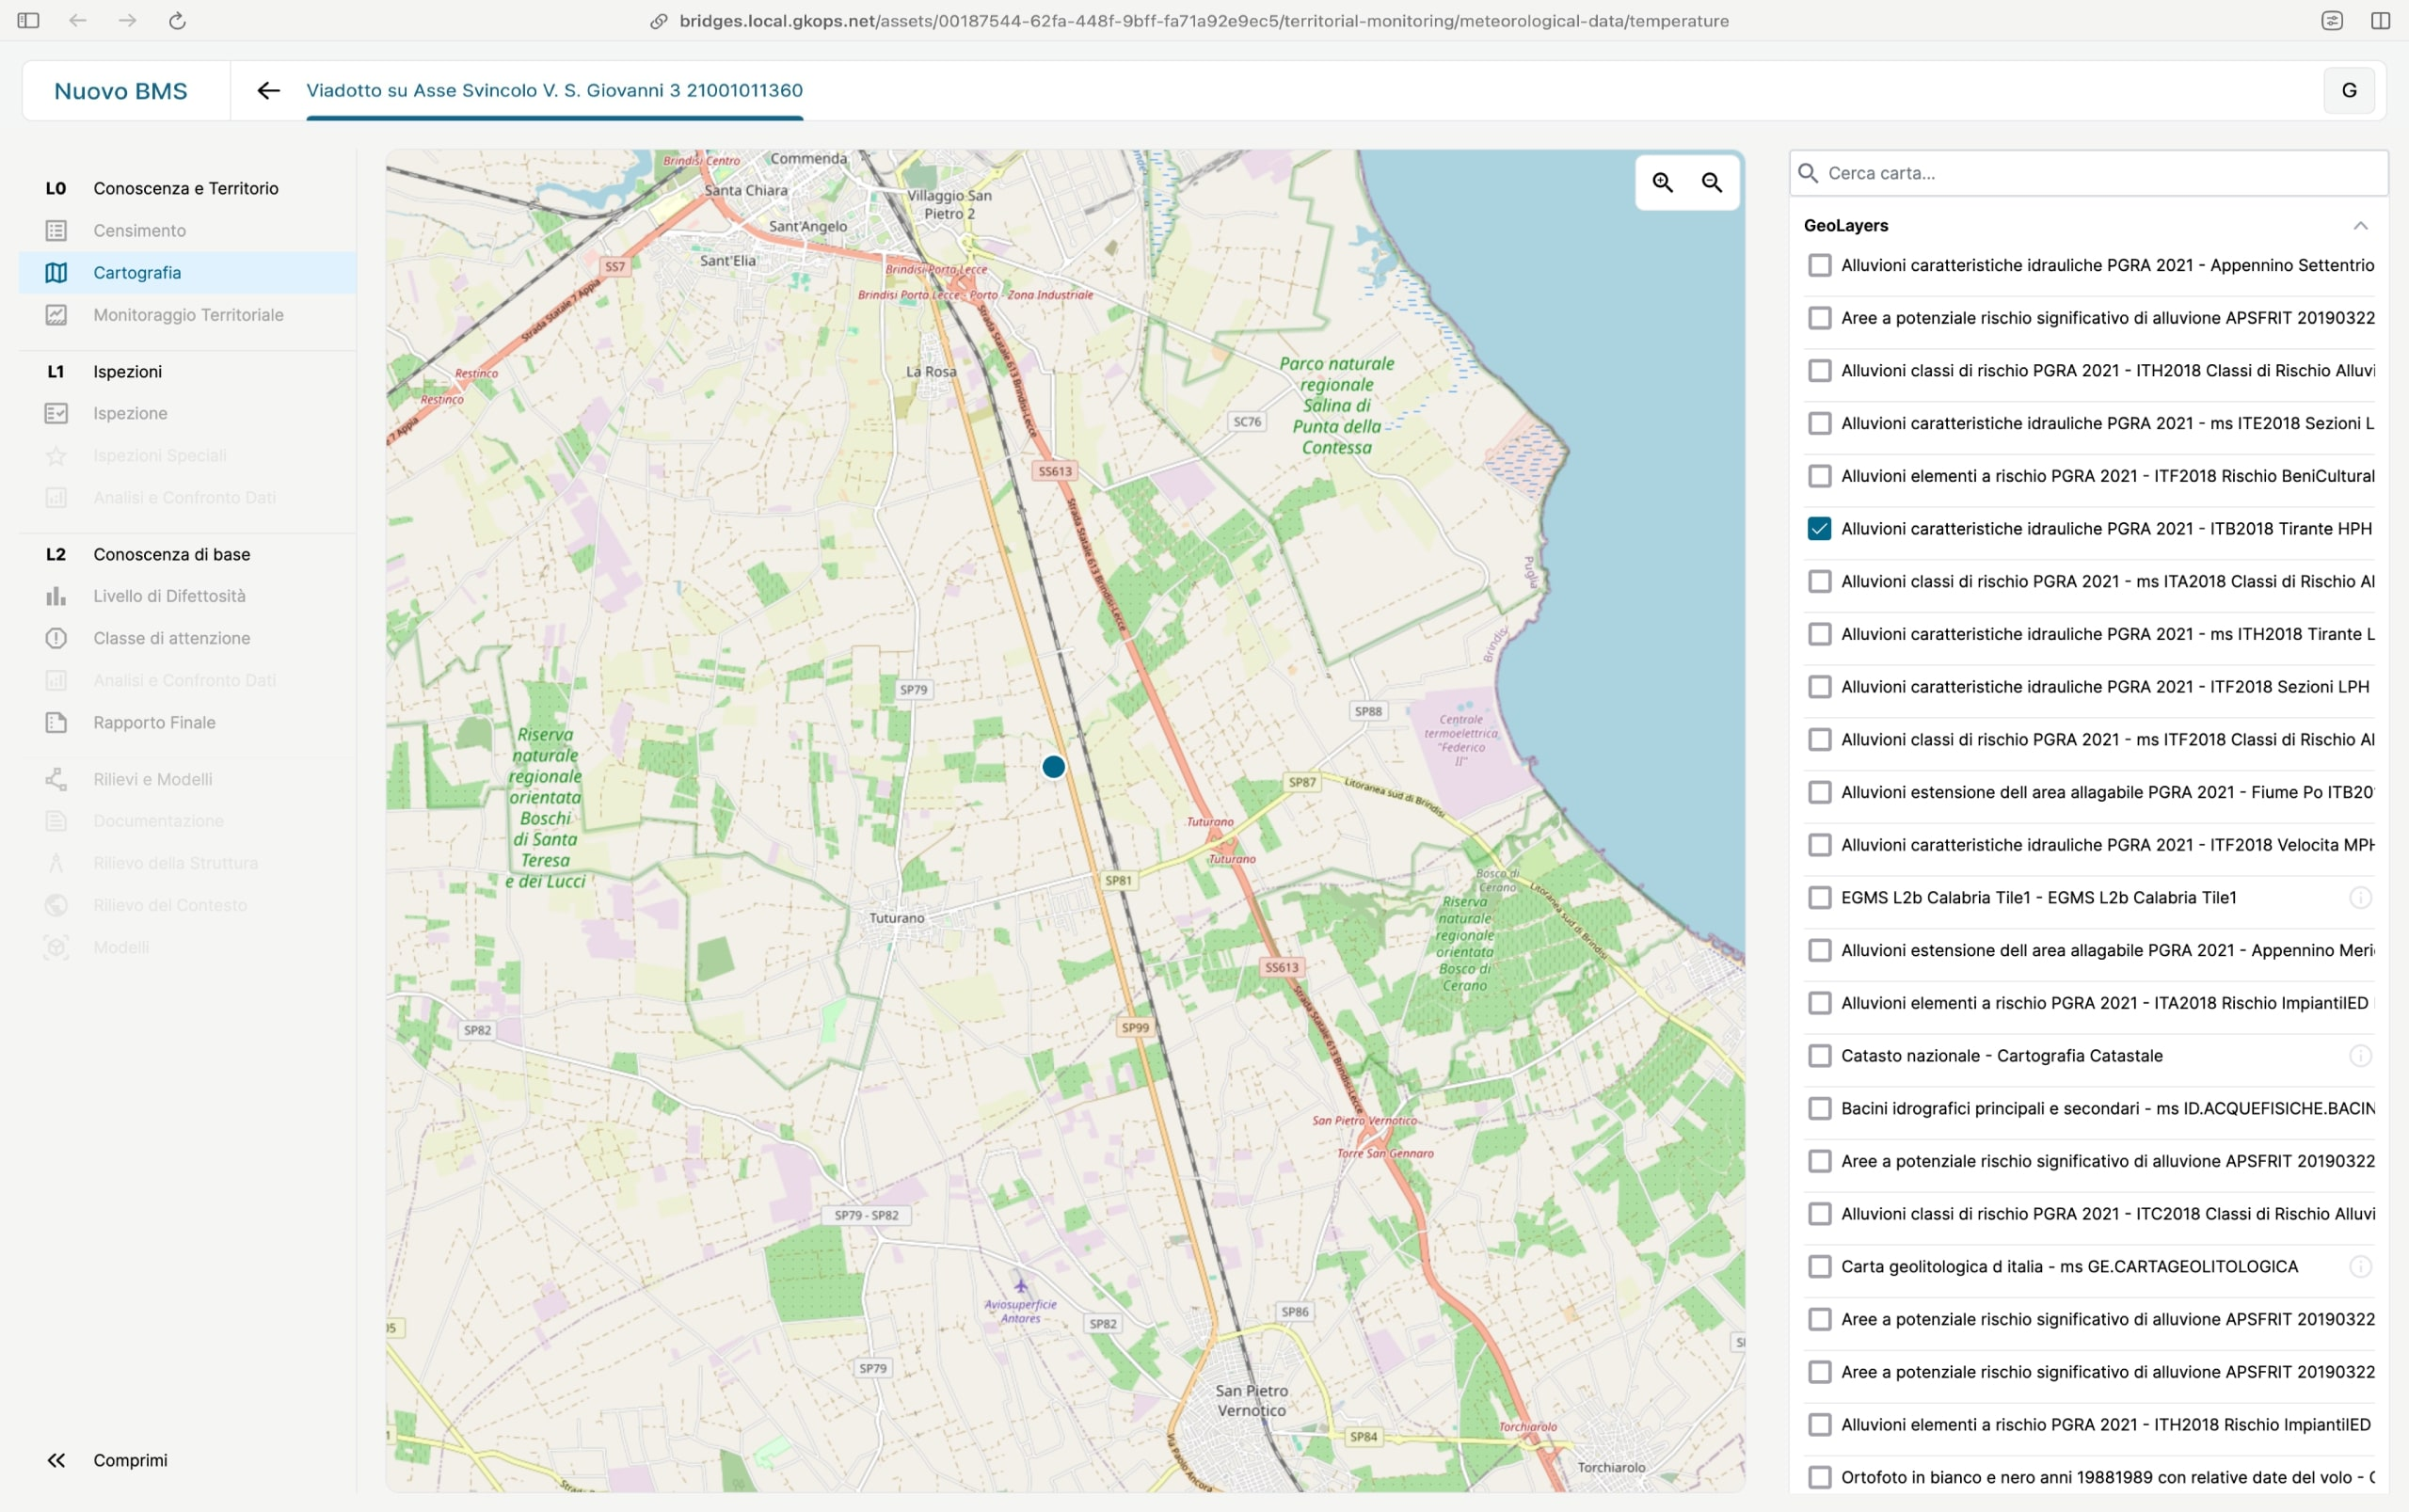
\includegraphics[width=1\textwidth]{Tesi/images/Capitolo7/listaMappe.jpg}
      \caption{Interfaccia grafica per mostrare la lista delle mappe}
      \label{fig:listaMappe}
\end{figure}
\\In conclusione, per spiegare meglio il ciclo di vita effettuato dal front-end e dal back-end, viene mostrato qui sotto l'elenco delle operazioni, eseguite in successione, al fine di ottenere il sistema funzionante:
\begin{enumerate}
    \item back-end: viene eseguito il comando \verb|to-geoserver| per caricare le mappe all'interno del server di mappe.
    \item back-end: viene eseguito il comando \verb|to-database| per inserire  le mappe all'interno del database.
    \item front-end: viene eseguita una richiesta HTTP in GET all'endpoint delle mappe, al fine di ottenere la lista.
    \item back-end: viene eseguita una query verso il database per ottenere la lista delle mappe disponibili.
    \item back-end: la Rest API risponde al client con la lista delle mappe, in formato JSON.
    \item front-end: il client legge il contenuto della lista e mostra graficamente l'elenco.
    \item front-end: quando viene selezionata una mappa, il client contatta il server di mappe per ottenerne i dati.
\end{enumerate}
